\section{analyzerbase.h File Reference}
\label{analyzerbase_8h}\index{analyzerbase.h@{analyzerbase.h}}


{\tt \#include $<$config.h$>$}\par
{\tt \#include \char`\"{}fht.h\char`\"{}}\par
{\tt \#include $<$qpixmap.h$>$}\par
{\tt \#include $<$qtimer.h$>$}\par
{\tt \#include $<$qwidget.h$>$}\par
{\tt \#include $<$vector$>$}\par


Include dependency graph for analyzerbase.h:\begin{figure}[H]
\begin{center}
\leavevmode
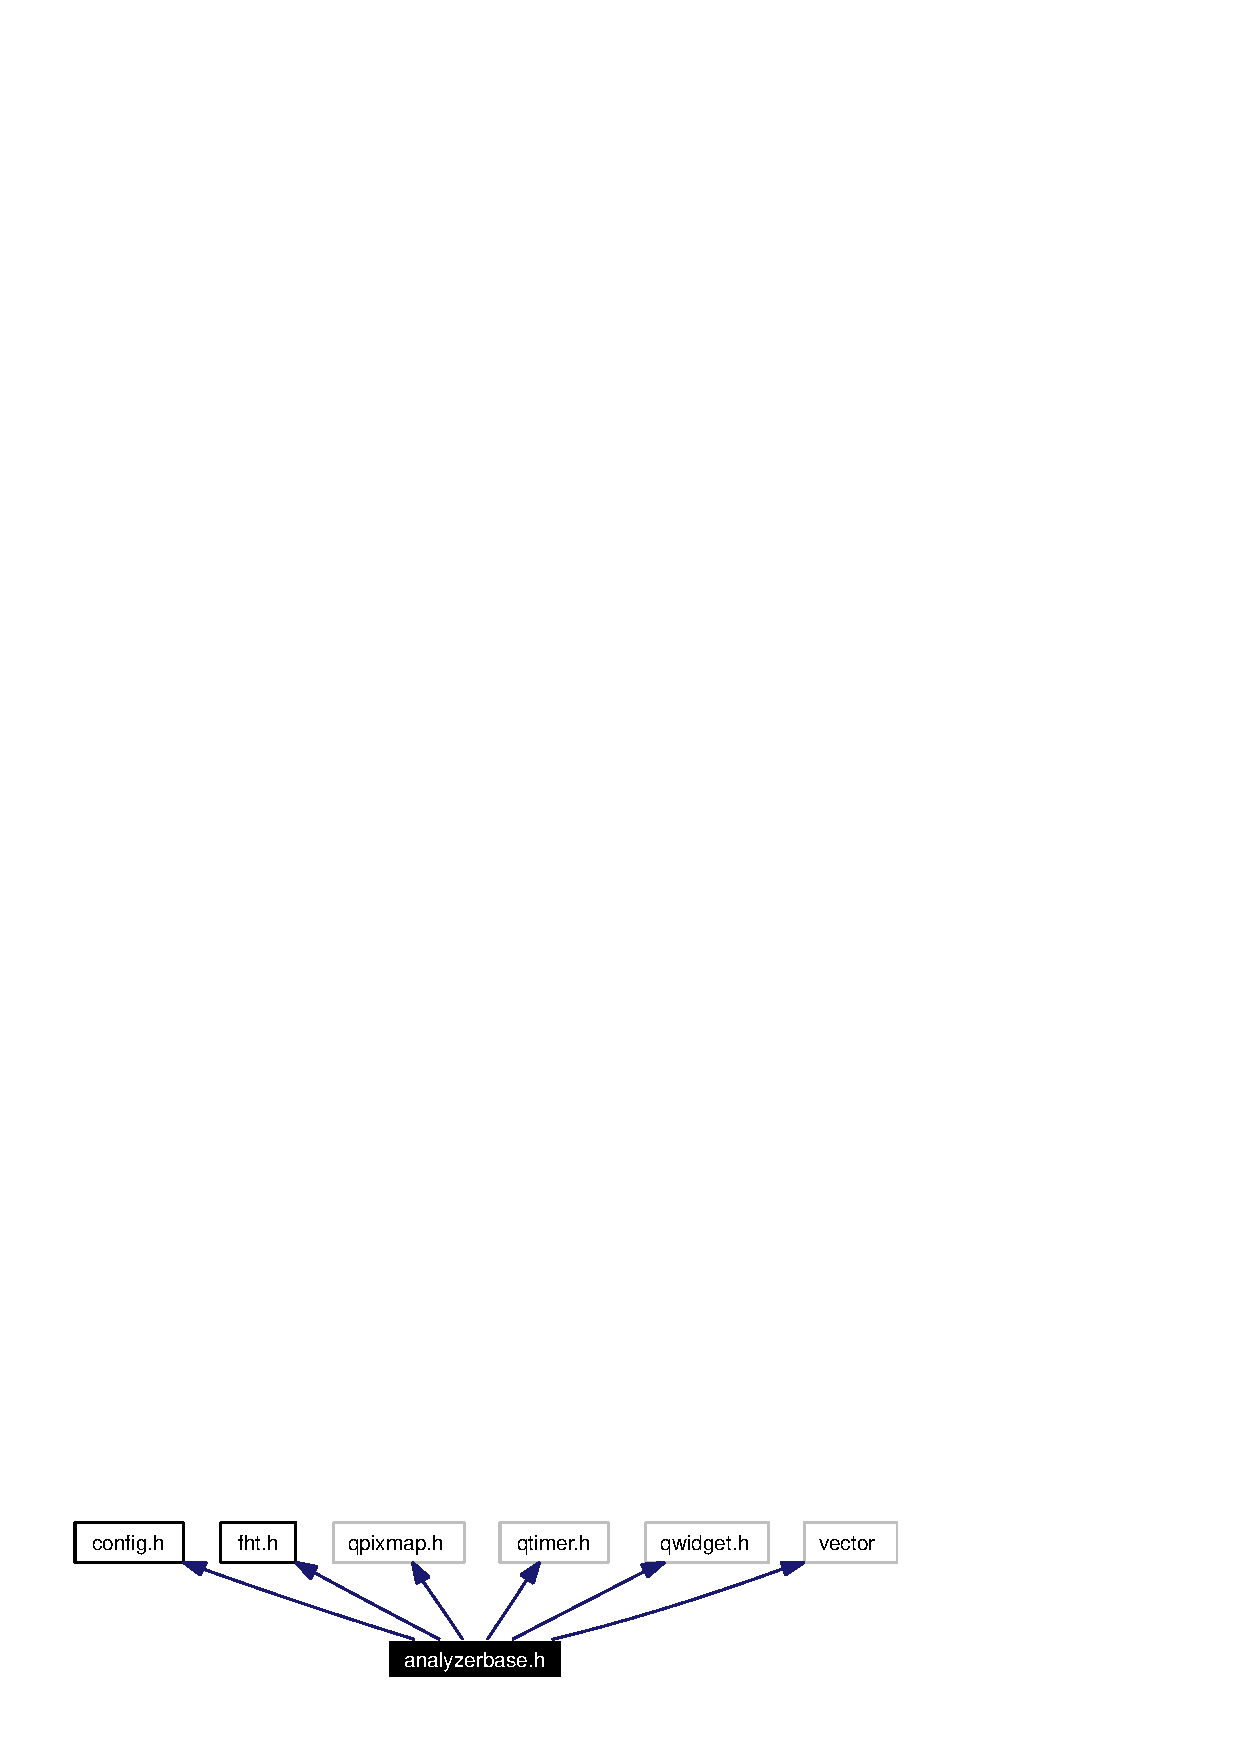
\includegraphics[width=215pt]{analyzerbase_8h__incl}
\end{center}
\end{figure}


This graph shows which files directly or indirectly include this file:\begin{figure}[H]
\begin{center}
\leavevmode
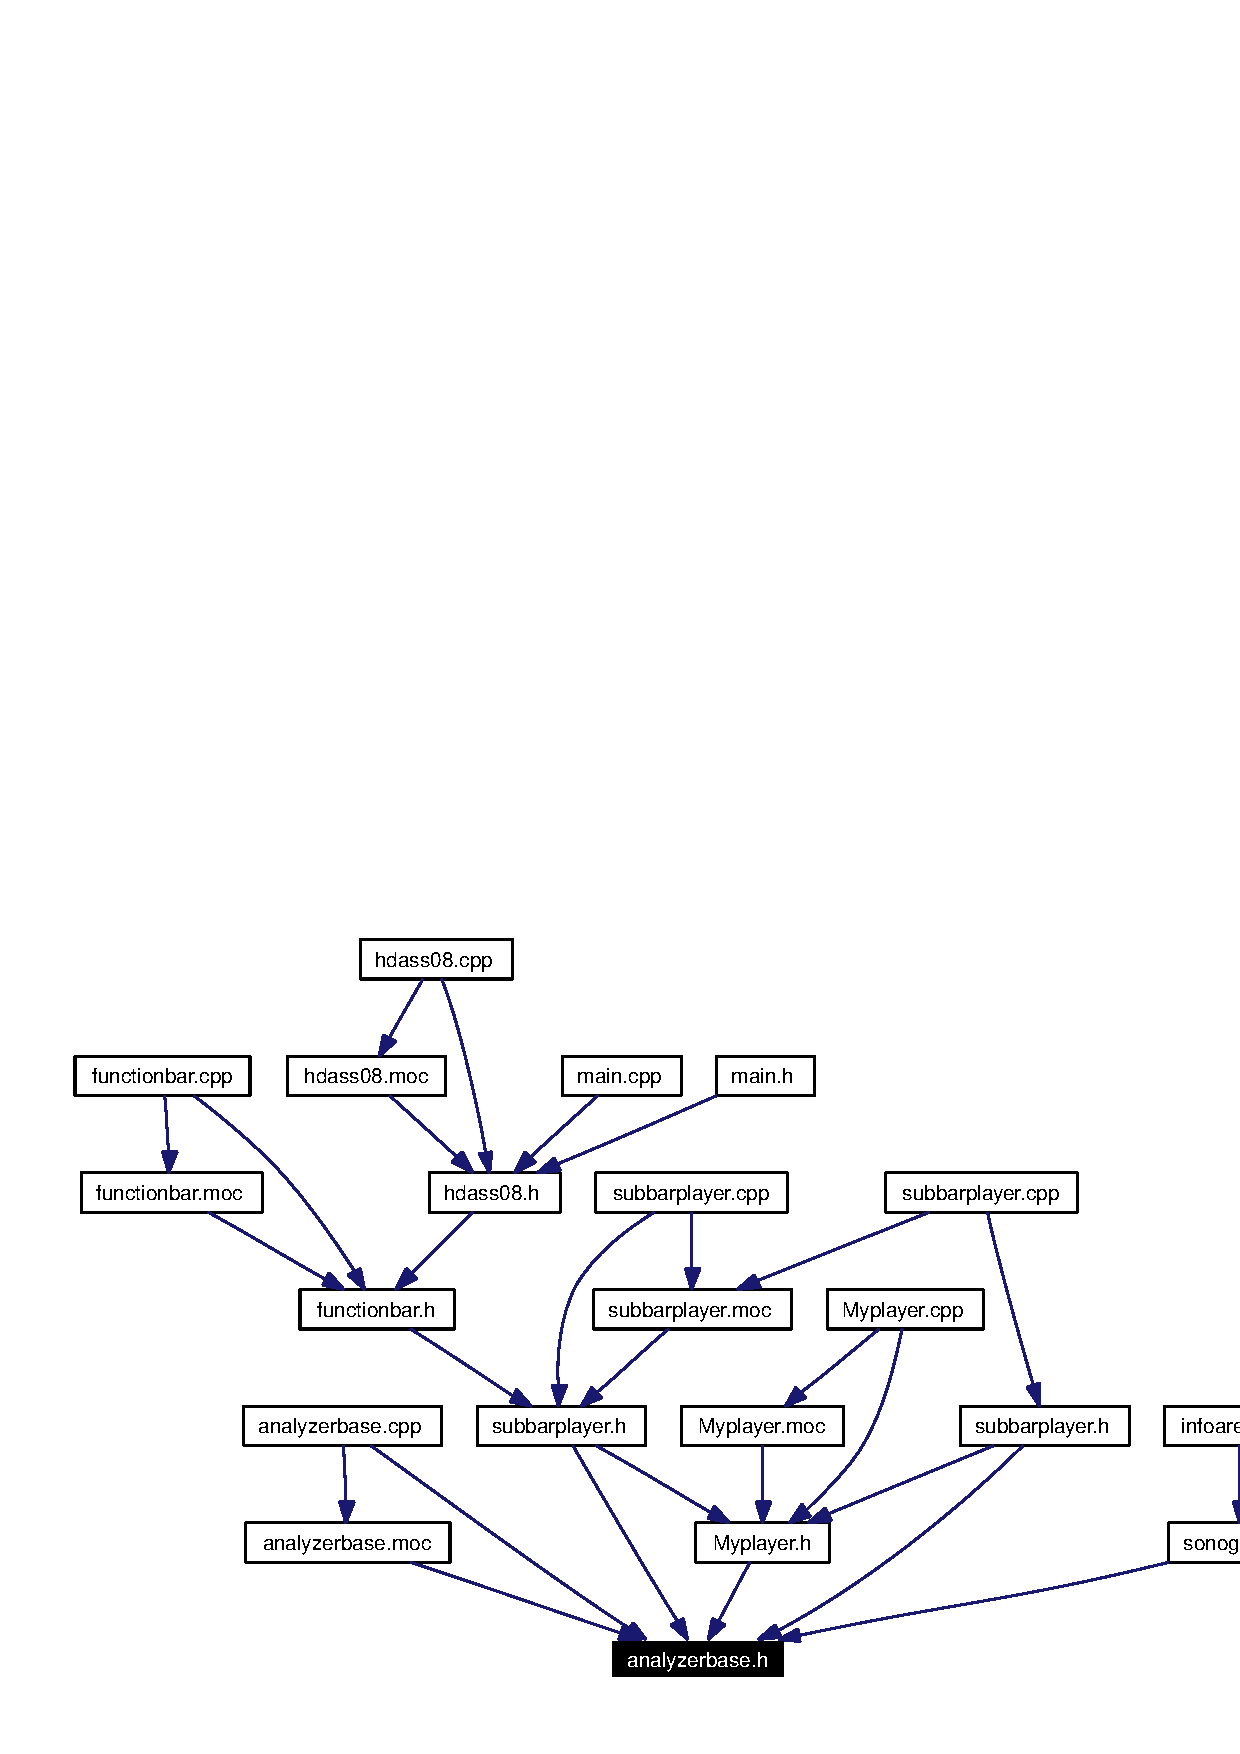
\includegraphics[width=365pt]{analyzerbase_8h__dep__incl}
\end{center}
\end{figure}
\subsection*{Namespaces}
\begin{CompactItemize}
\item 
namespace {\bf Analyzer}
\end{CompactItemize}
\subsection*{Defines}
\begin{CompactItemize}
\item 
\#define {\bf QGLWidget}\ {\bf QWidget}
\end{CompactItemize}


\subsection{Define Documentation}
\index{analyzerbase.h@{analyzerbase.h}!QGLWidget@{QGLWidget}}
\index{QGLWidget@{QGLWidget}!analyzerbase.h@{analyzerbase.h}}
\subsubsection{\setlength{\rightskip}{0pt plus 5cm}\#define {\bf QGLWidget}\ {\bf QWidget}}\label{analyzerbase_8h_a0}




Definition at line 24 of file analyzerbase.h.